\chapter{GIS基础知识介绍}

GIS的基础知识

\begin{itemize}
	\item 坐标
	      \begin{itemize}
		      \item 二维坐标: 点坐标、线坐标、区坐标
		      \item 三维坐标:球坐标、面坐标、体坐标
	      \end{itemize}
	\item 投影变换
	      \begin{itemize}
		      \item EPSG\footnote{European Petroleum Survey Group-欧洲石油调查组织}:4326-经纬度投影\footnote{\href{http://epsg.io/4326}{EPSG:4326} }
		      \item EPSG:3857-WEB墨卡托投影\footnote{\href{http://epsg.io/3857}{EPSG:3857} }
	      \end{itemize}
\end{itemize}

\section{坐标}

坐标分为二维坐标(x, y)和三维坐标(x, y, z)

\begin{enumerate}
	\item \textbf{x}:表示横轴坐标,地理上表示经度
	\item \textbf{y}:表示纵轴坐标,地理上表示纬度
\end{enumerate}

% https://www.latexstudio.net/archives/51453.html
% https://en.wikibooks.org/wiki/LaTeX/PGF/TikZ
\begin{tikzpicture} [scale=2]
	\draw[step=1,color=gray!40] (-2,-1) grid (2,1);
	\draw[->] (-3,0) -- (3,0) node[right] {$x$};
	\draw[->] (0,-2) -- (0,2) node[right] {$y$};
	\draw[red] (10:1cm) (-2, 0) -- (2, 0) node[right] {赤道};
	\draw[blue] (10:1cm) (0,-1) -- (0,1) node[align=center] {本初子午线};
	\draw[dotted] (-2,1) node {西北 -180,90 };
	\draw[dotted] (2,1) node {东北 180, 90};
	\draw[dotted] (-2,-1) node {西南 -180 -90};
	\draw[dotted] (2,-1) node {东南 180 -90};
	\draw[dotted] (2,1) node {东北 180, 90};
	\draw[dashed, red, ->] (1,0.5) -- (1,0);
	\draw[dashed, blue, ->] (1,0.5) -- (0,0.5);
	\draw[dotted, red] (1,0.5) node {(90, 45)};
\end{tikzpicture}

\begin{note}
	以我们家地理坐标为例(114.372680, 30.404060)为例子。其在形态上有多中表示方式
	\begin{itemize}
		\item 点坐标-中心点-(114.372680, 30.404060)在真实地理空间上表示的点的位置,即经纬度,作用是快速的抽象成一个点几何。
		\item 线坐标-轮廓
		      \begin{lstlisting}
    "geometry": {
    "type": "LineString",
    "coordinates": [
        [ 114.37035799026489, 30.404175106694034 ],
        [ 114.37033653259276, 30.403832731325604 ],
        [ 114.37238574028015, 30.403804971107995 ],
        [ 114.37235355377197, 30.40416585332147 ],
        [ 114.37203168869019, 30.40419361343649 ],
        [ 114.37204241752625, 30.404304653817682 ],
        [ 114.37184929847717, 30.404304653817682 ],
        [ 114.37183856964111, 30.40419361343649 ],
        [ 114.37086224555969, 30.40419361343649 ],
        [ 114.37086224555969, 30.404323160535583 ],
        [ 114.37052965164185, 30.404332413893236 ],
        [ 114.37051892280579, 30.404184360065706 ],
        [ 114.37035799026489, 30.404175106694034 ]
    ]
  }
  \end{lstlisting}
		      \begin{figure}[!htb]
			      \centering
			      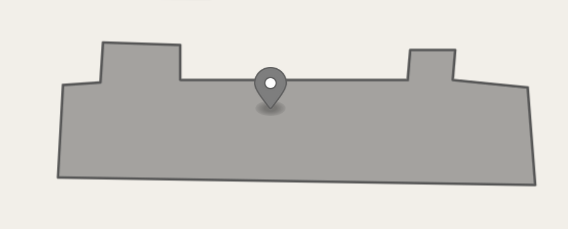
\includegraphics[width=0.9\textwidth]{./charpter1/my_home.png}
		      \end{figure}
		\item 区坐标-最小外包矩形
		      \begin{figure}[!htb]
			      \centering
			      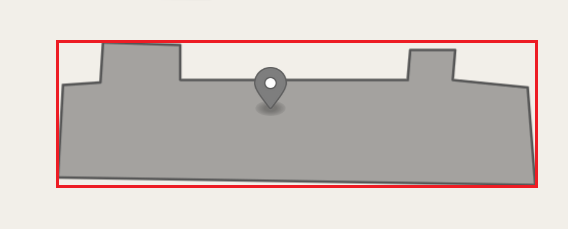
\includegraphics[width=0.9\textwidth]{./charpter1/my_home_bounds.png}
		      \end{figure}
	\end{itemize}
\end{note}



\section{投影变换}
投影变换是将真实的三维的椭球的地球显示投影成平面的二维地图上。
以国内常用的的二中投影来进行介绍:
\begin{enumerate}
	\item 等分弧秒投影
	\item 墨卡托投影(Mercator Projection)
	\item 高斯-克吕格投影(Transverse Mercator Projection)
\end{enumerate}
投影变换的本质是将\textbf{真实三维的(x, y, z) 投放到平面二维的(x, y)上}。

\subsection{墨卡托投影}
墨卡托的投影原理是正轴等角圆柱投影\footnote{https://en.wikipedia.org/wiki/Mercator\_projection}。
\begin{figure}[!htb]
	\centering
	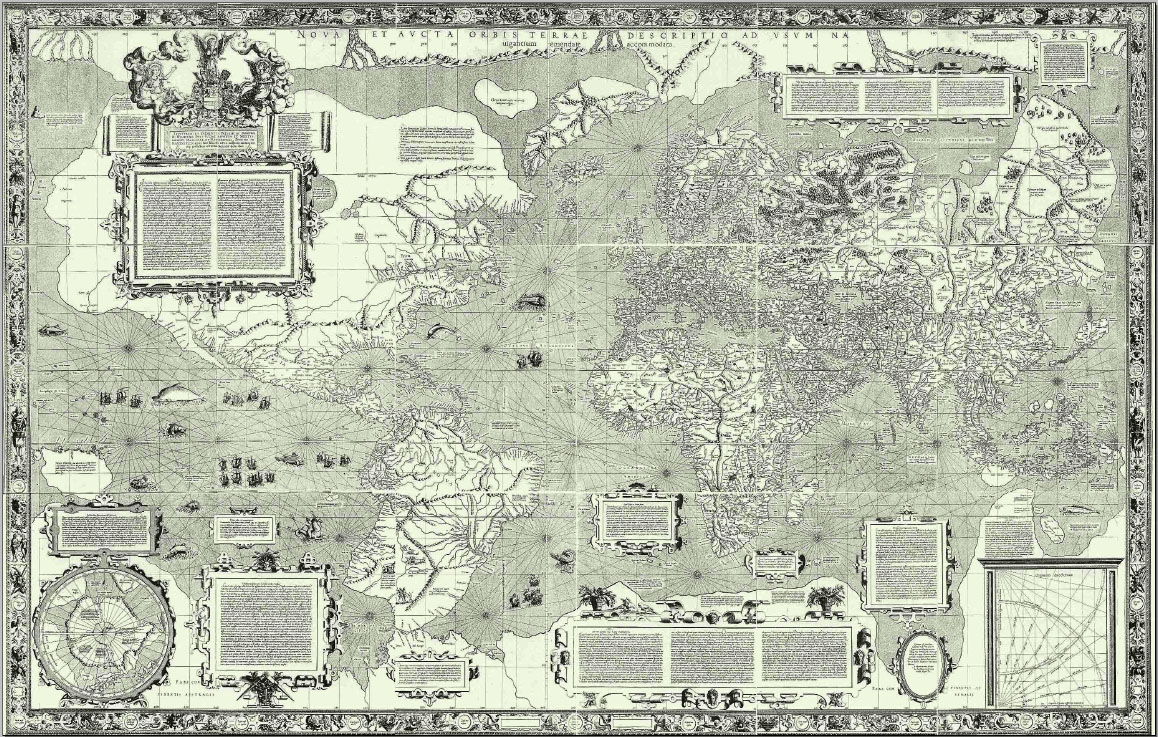
\includegraphics[width=0.9\textwidth]{./charpter1/Mercator_1569.png}
\end{figure}
1569年的墨卡托投影\footnote{https://en.wikipedia.org/wiki/Mercator\_1569\_world\_map}


\begin{figure}[!htb]
	\centering
	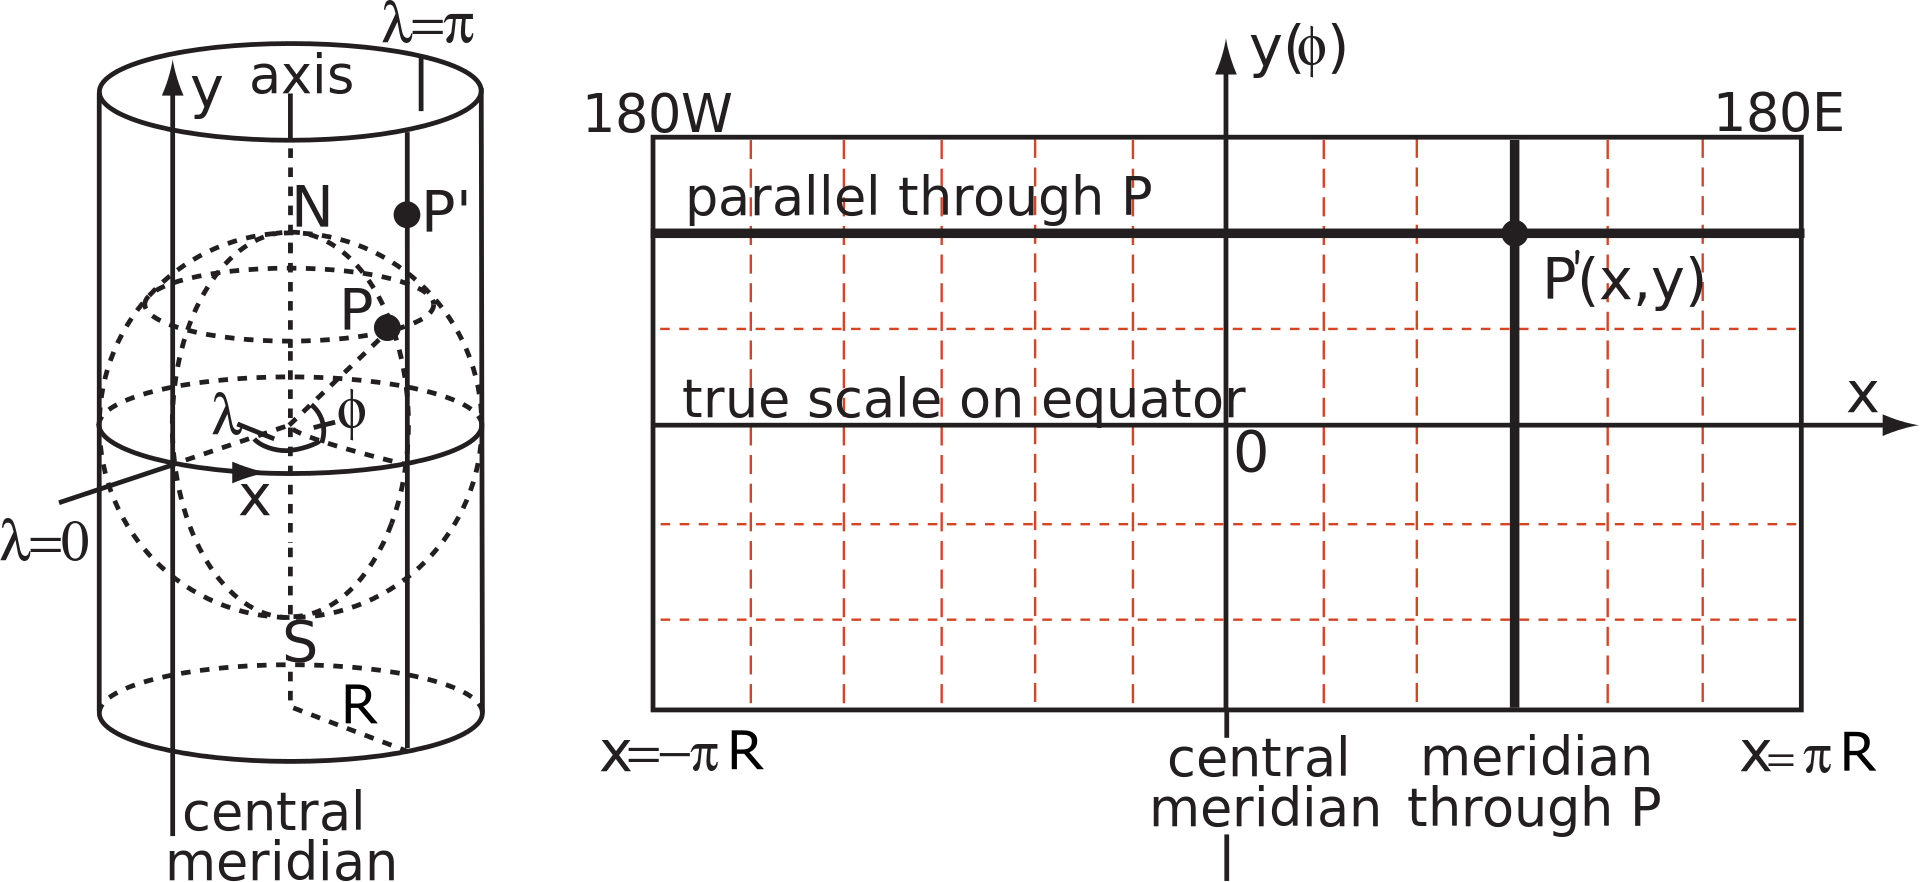
\includegraphics[width=0.9\textwidth]{./charpter1/Cylindrical_Projection_basics2.png}
\end{figure}
图中的一个实际地球表面上的点P经过投影变换后投射到圆柱平面上的点P'
\begin{enumerate}
	\item 经度λ:
	\item 纬度φ:
	\item x轴:经度经过投影函数x(λ)后计算得出对应的值
	\item y轴:纬度经过投影函数y(φ)后计算得出对应的值
\end{enumerate}

\begin{note}
	这里绝对不能把该场景想象从地心发射一条光线从P点穿透出来射到圆柱上形成点P',这个是错误的计算方式和思维模拟。
\end{note}

\subsection{高斯-克吕格投影}
高斯-克吕格投影的投影原理是等角横切椭圆柱投影。
TM\footnote{https://en.wikipedia.org/wiki/Transverse\_Mercator\_projection}
UTM\footnote{https://en.wikipedia.org/wiki/Universal\_Transverse\_Mercator\_coordinate\_system}
记得我在学习的时候,课本上讲解的都是类似西瓜皮的投影方式,当时只是从大概上了解了其原理。我相信和我一样有着疑问的人不在少数。本章节将从工程角度上详细剖解其数学原理。
\begin{figure}[!htb]
	\centering
	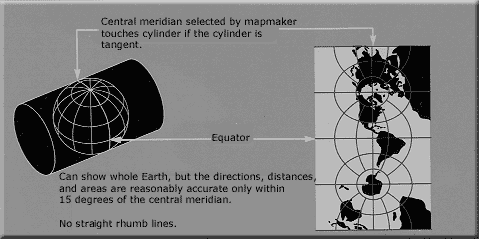
\includegraphics[width=0.9\textwidth]{./charpter1/Usgs_map_traverse_mercator.png}
\end{figure}



\section{切分模型}
由于一次性传输大量的矢量数据会导致性能瓶颈,因此需要针对海量数据进行LOD\footnote{多层次细节,Level Of Detail}处理.

\subsection{切分原理}
切分的基本原理是将整个世界
\begin{figure}[!htb]
	\centering
	% https://www.latexstudio.net/archives/51453.html
	% https://en.wikibooks.org/wiki/LaTeX/PGF/TikZ
	% https://graphviz.org/doc/info/shapes.html
	\begin{tikzpicture} [scale=2]
		\draw[step=1,color=gray!40] (-2,-1) grid (2,1);
		\draw[->] (-3,0) -- (3,0) node[right] {$x$};
		\draw[->] (0,-2) -- (0,2) node[right] {$y$};
		\draw[red] (10:1cm) (-2, 0) -- (2, 0) node[right] {赤道};
		\draw[blue] (10:1cm) (0,-1) -- (0,1) node[align=center] {本初子午线};
		\draw[dotted] (-2,1) node {西北 -180,90 };
		\draw[dotted] (2,1) node {东北 180, 90};
		\draw[dotted] (-2,-1) node {西南 -180 -90};
		\draw[dotted] (2,-1) node {东南 180 -90};
		\draw[dotted] (2,1) node {东北 180, 90};
		\draw[dashed, red, ->] (1,0.5) -- (1,0);
		\draw[dashed, blue, ->] (1,0.5) -- (0,0.5);
		\draw[dotted, red] (1,0.5) node {(90, 45)};
	\end{tikzpicture}
	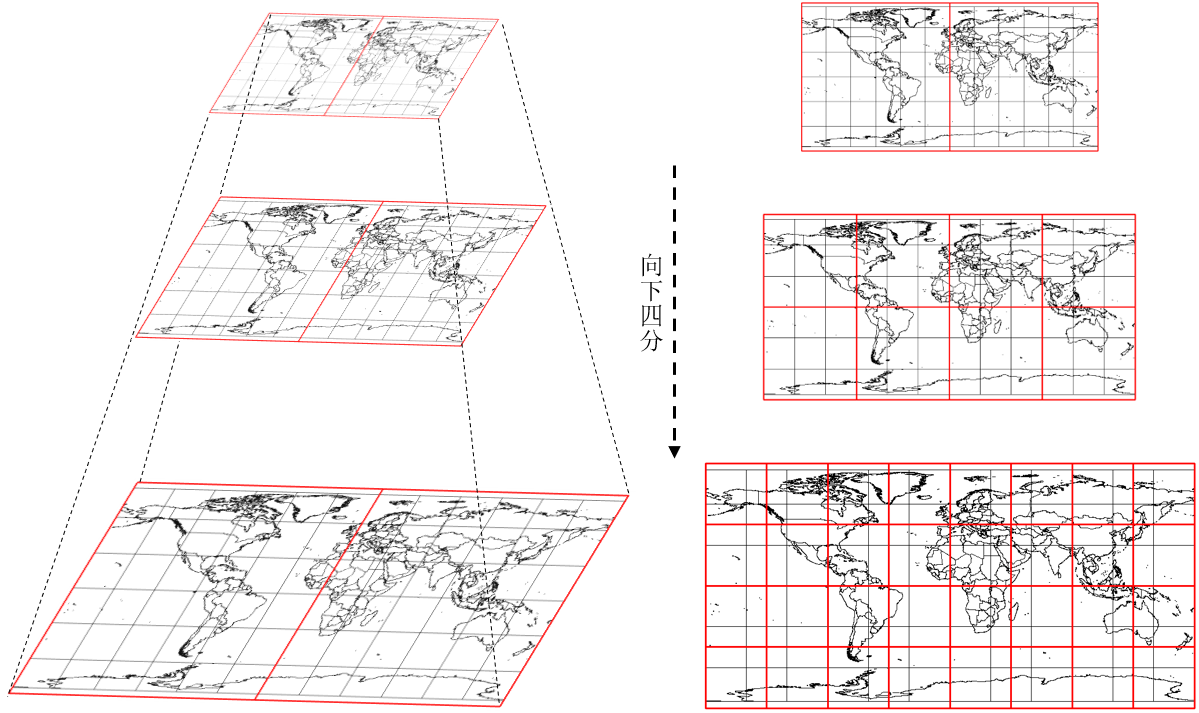
\includegraphics[width=0.9\textwidth]{./charpter1/lonlat_tilegrid.png}
\end{figure}

\subsection{切分规则}

瓦片矩阵集由多个瓦片矩阵集合组成,每个瓦片矩阵都有一个分辨率针对特定比例进行优化,并由\textbf{TileMatrix}标识符标识。
% 每个贴图矩阵集都有一个可选的近似边界框,但每个贴图矩阵都有间接从其他参数推导出的精确边界框。
瓷砖矩阵由于像素对齐,每个比例的包围框通常会略有不同对于客户机和服务器来说,考虑这种变化是很重要的。
在左上角瓷砖矩阵在CRS坐标中的点(tileMatrixMinX, tileMatrixMaxY),
宽度和瓦片矩阵的高度,以瓦片单位(matrixWidth, matrixHeight),
宽度和贴图的高度,以像素为单位(tileWidth, tileHeight),
转换坐标的系数参考系统(CRS)的单位分为米(metersPerUnit)
和比例尺(1: scalednominator),
贴图矩阵的边界框的右下角(tileMatrixMaxX, tileMatrixMinY)可计算如下:

OGC WMTS标准中DPI是90.71,即采用0.028mm作为一个像素的物理宽度,与天地图规范不一致(规范中DPI为96)。
前端程序调用WMTS接口获取元信息后,需要根据元信息中的比例尺和DPI参数重新计算瓦片分辨率。
理论上,天地图或支持天地图的相关产品DPI值都应该为96。
ArcGIS等商业软件的DPI值默认采用OGC标准中的90.71。


DPI(每英寸多少像素点) = dots / inch  = 90.71 dpi; \\
1 英寸 = 25.4 毫米 \\
DPMM(每毫米多少像素点) = dots / millimeter =  DPI * (millimeter / inch) = 25.4 / 90.71 = 0.28;

\begin{align}
	scale = 1 inch                                                    \\
	pixelSpan = scaleDenominator \times 0.28 \div metersPerUnit(crs); \\
	tileSpanX = tileWidth \times pixelSpan;                           \\
	tileSpanY = tileHeight \times pixelSpan;                          \\
	tileMatrixMaxX = tileMatrixMinX + tileSpanX \times matrixWidth;   \\
	tileMatrixMinY = tileMatrixMaxY - tileSpanY \times matrixHeight;
\end{align}

\begin{figure}[!htb]
	\centering
	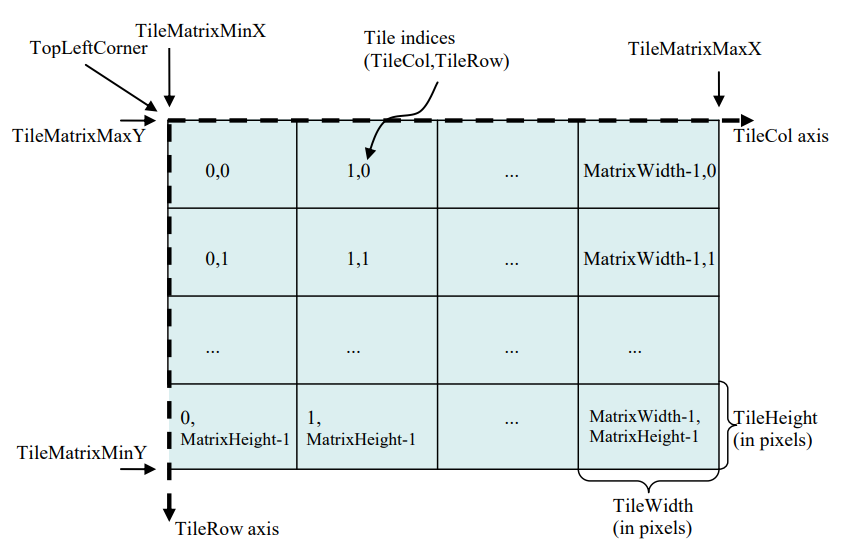
\includegraphics[width=0.55\textwidth]{./charpter1/ogc_tilegrid.png}
	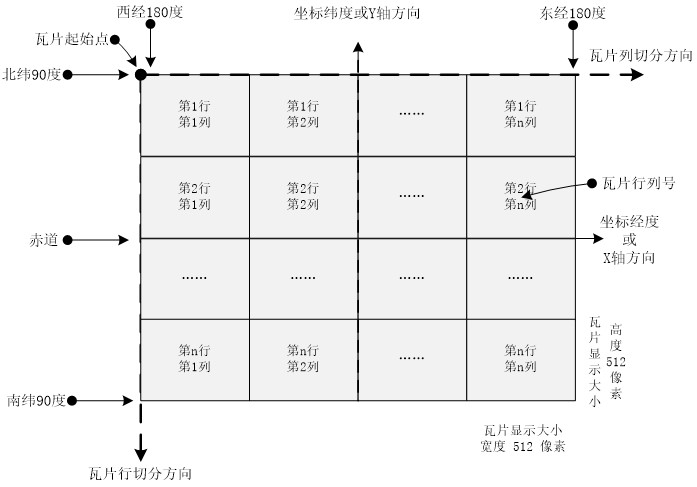
\includegraphics[width=0.55\textwidth]{./charpter1/math_tilegrid.jpg}
\end{figure}

\subsection{常见切分规范}
\begin{itemize}
	\item EPSG:4326 等分弧秒投影 \footnote{地理坐标系统(Geographical Coordinate System), 经纬度直投, 近似是说的同一个东西,这里该投影属于一种任意投影,不太严谨,不做学术上争论 , http://epsg.io/4326}
	\item EPSG:3857 Web墨卡托投影 \footnote{投影坐标系统 (Projection Coordinate System) http://epsg.io/3857}
\end{itemize}

\subsubsection{等分弧秒投影}
\label{sec:lonlat-project}
经纬度等分弧秒投影后的世界地图为南北短,东西宽的矩形。选择在经度0方向进行切割,使得全球地图是两张在经纬度方向长宽相等的正方形矩形区域。全球制图范围为纬度 [-90, 90],经度[-180, 180]。
\begin{itemize}
	\item Cesium地形\footnote{\hyperref[sec:cesium-terrain]{跳转至Cesium地形章节}}默认采取该投影
	\item Cesium栅格\footnote{\hyperref[sec:cesium-raster]{跳转至Cesium栅格章节}}可以通过\textbf{GeographicTilingScheme}加载经纬度坐标系瓦片
\end{itemize}

\begin{figure}[!htb]
	\centering
	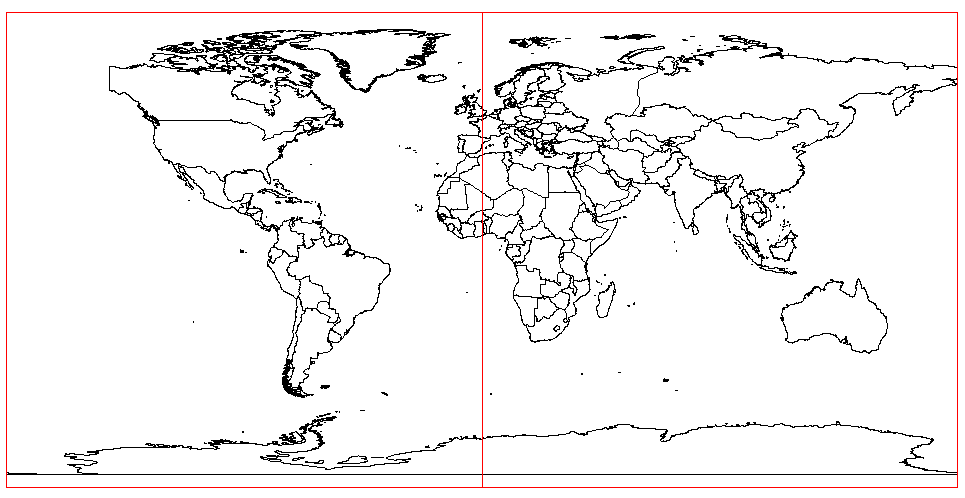
\includegraphics[width=0.8\textwidth]{./charpter1/tile/lonlat-level-1.png}
\end{figure}
\subsubsection{Web墨卡托投影}
Web墨卡托投影后的世界地图为南北略长,东西略窄的矩形,选择在纬度+-85.051128度进行切割,使得全球地图是一张在经纬度方向长宽相等的正方形区域。此时全球制图范围为纬度[-85.051128, 85.051128], 经度[-180, 180],投影后平面坐标范围为:X[-20037508.34米, 20037508.34米], Y[-20037508.34米, 20037508.34米]。
\hyperref[sec:cesium-terrain]{Cesium栅格默认采取该投影}
\begin{itemize}
	\item Cesium栅格\footnote{\hyperref[sec:cesium-raster]{跳转至Cesium栅格章节}}默认采取该投影
	\item MapboxGL栅格默认采取该投影
\end{itemize}
\begin{figure}[!htb]
	\centering
	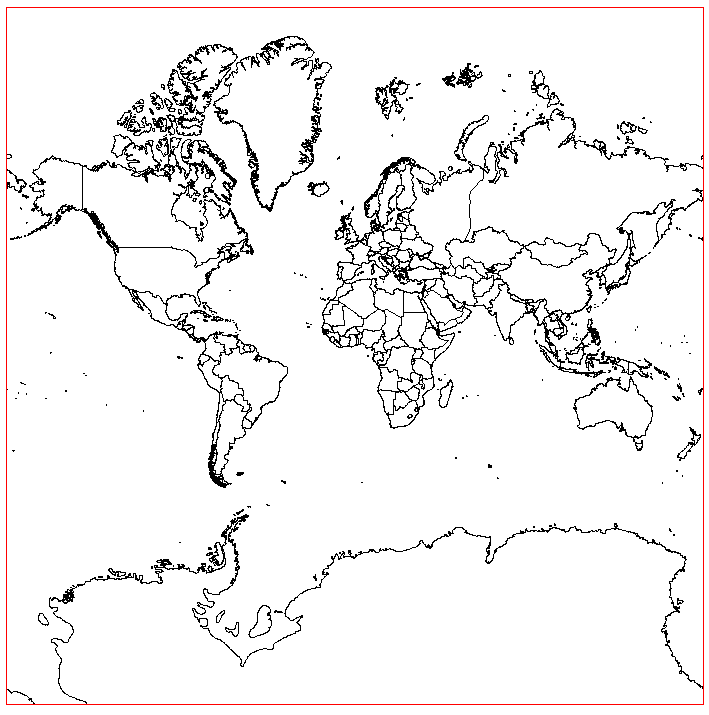
\includegraphics[width=0.5\textwidth]{./charpter1/tile/mkt-level-1.png}
\end{figure}
\subsubsection{投影组合}
\textbf{Cesium投影组合}

\begin{introduction}
	\item Cesium地形\textbf{默认采取等分弧秒投影}
	\item Cesium栅格\textbf{默认采取Web墨卡托投影}
	\item 投影坐标直接叠加显示 ? 否
	\item 矩阵变换叠加显示 ? 是
\end{introduction}
不知道细心的读者有没有上2章的细节中发现一个现象。那如果都走默认的前提下,岂不是2种投影叠加到一起的显示方式吗?
\begin{figure}[!htb]
	\centering
	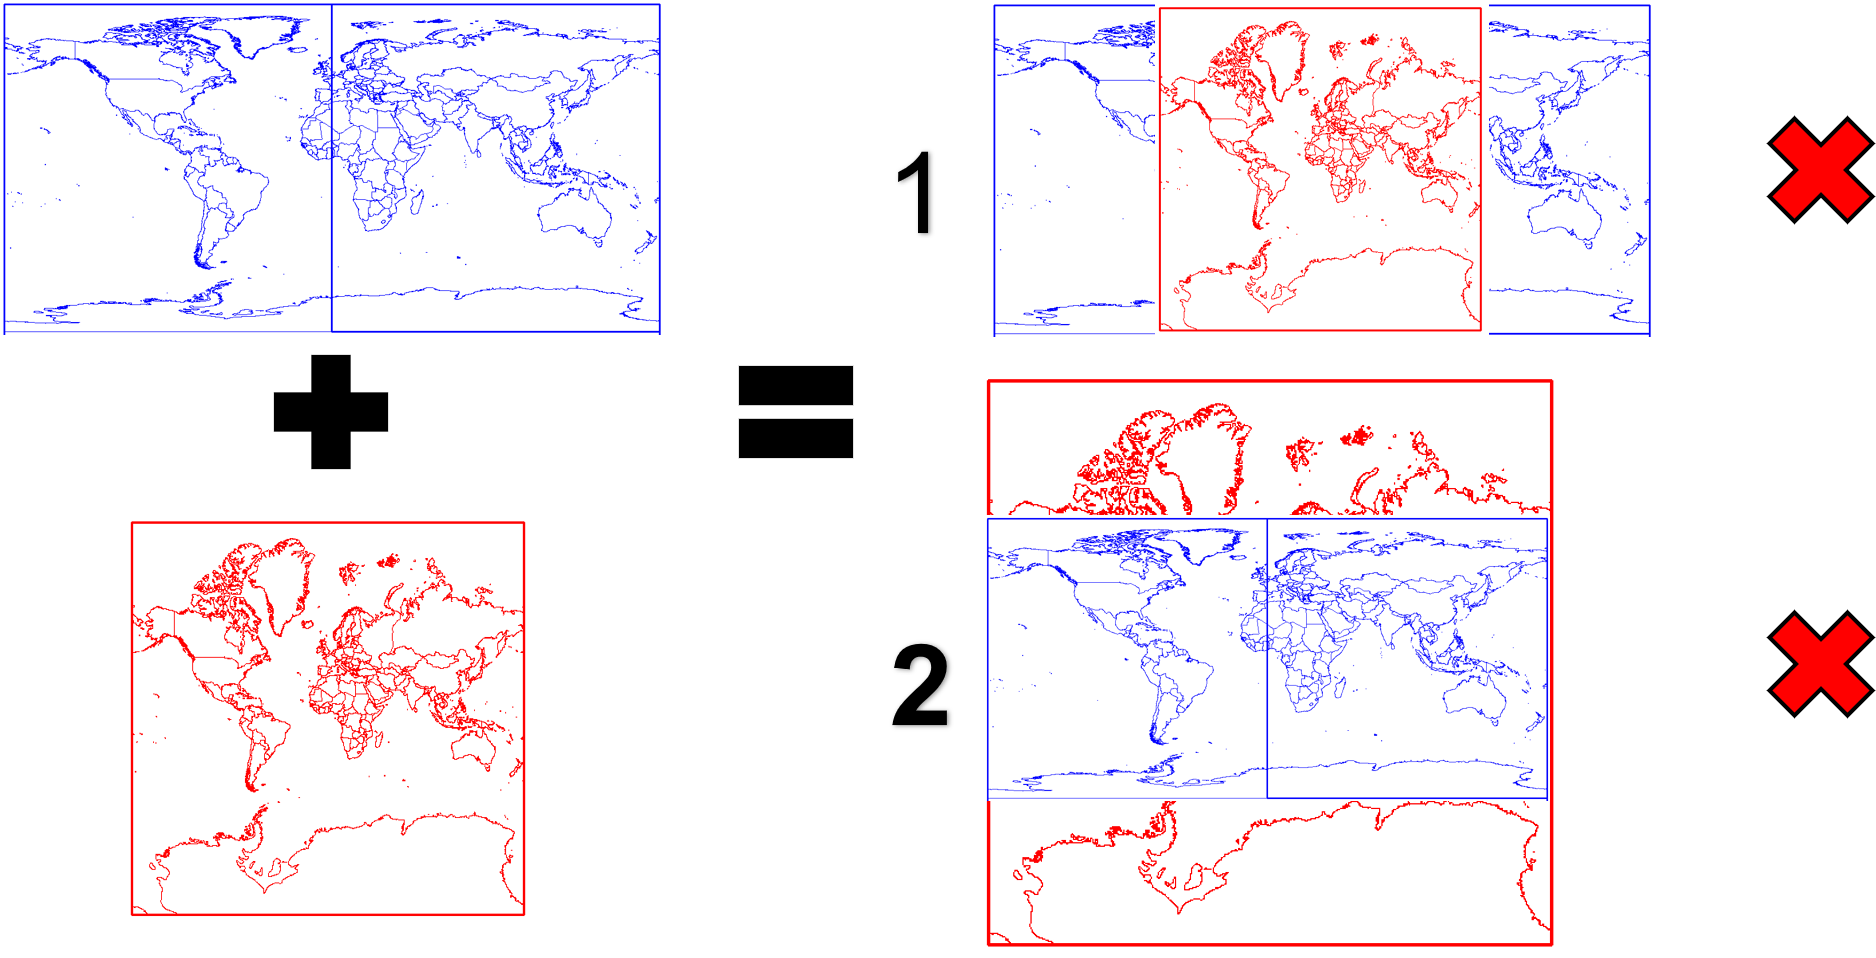
\includegraphics[width=1.0\textwidth]{./charpter1/project/error_combine.png}
\end{figure}
\begin{note}
	如上图所示,两种方式都无法通过简单的平移或者拉伸的方式来套合在一起。
\end{note}

\textbf{MapboxGL投影组合}

\section{变换}
上一节的投影讲解了如何把一个三维球形的投影到二维的平面上。但是实际场景中,可能需要进行一些放大,平移,旋转操作。
\begin{note}
	这一系列类操作在WebGL中通常称作模型变换。
\end{note}

\begin{enumerate}
	\item 放大操作,以某点为中心,按照比例进行缩放。
	\item 平移操作,以某点为中心,按照距离进行平移。
	\item 旋转操作,以某点为中心,按照角度进行旋转。
	\item 组合以上3中操作。
\end{enumerate}

\subsection{旋转操作}

\begin{SCfigure}
	\centering
	\caption{原始图像.左图如果是呈现在屏幕上,由于绝大部分的屏幕是宽大于高,因此该图形的左右侧会出现很多的空隙,
		因此在观感上表现会很稀疏。因此如果能够把该图形旋转90度后横着放,就可以省下很多的空间了。
		那如何旋转呢,是以左上角还是右上角还是左下角还是右上角呢,这里我们先选择最容易理解的中心点来演示。
		图中的绿色点表示中心点。}
	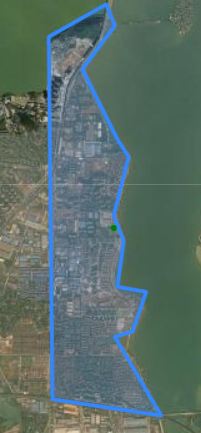
\includegraphics[width=0.3\textwidth]{./charpter1/transform/before_rotate.png}
\end{SCfigure}

\begin{figure}[!htb]
	\centering
	\caption{旋转后的位置如图所示}
	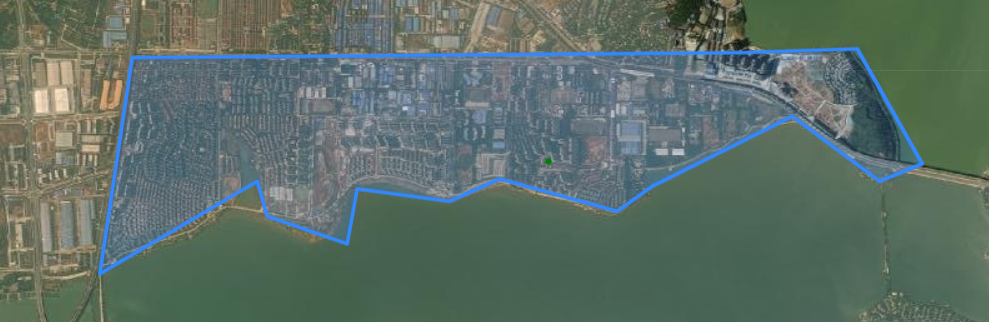
\includegraphics[width=0.8\textwidth]{./charpter1/transform/after_rotate.png}
\end{figure}

\subsection{数学原理}
\begin{figure}[!htb]
	\centering
	\caption{图形原理}
	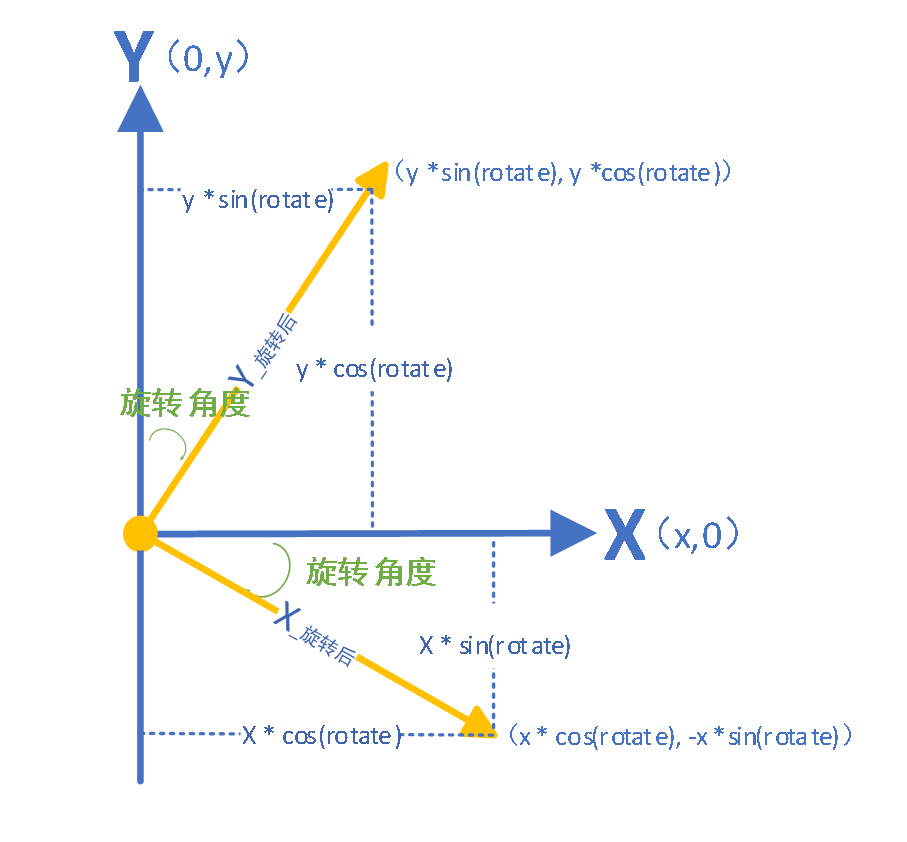
\includegraphics[width=0.8\textwidth]{./charpter1/transform/rotate.png}
\end{figure}

上图可以知道得到的原来的正常的的X,Y通过旋转角度 $\alpha$ 后得到的新的$X'$, $Y'$如下所示:

\begin{subequations}
	\begin{align}
		X & =(x, 0) \\
		Y & =(0, y)
	\end{align}
\end{subequations}

\begin{subequations}
	\begin{align}
		X' & =(x \times \cos \alpha, -x \times \sin \alpha) \\
		Y' & =(y \times \sin \alpha, y \times \cos \alpha)
	\end{align}
\end{subequations}

上面的公式知道了原始的X,Y的基向量,也求出了旋转后的X',Y'的基向量。
因此原始X,Y中的向量$\overrightarrow{A}$,在新坐标系X',Y'后得到的$\overrightarrow{A'}$值为
	\begin{subequations}
		\begin{align}
			\overrightarrow{A} & = (a, b) \\
			X' & =(x \times \cos \alpha, -x \times \sin \alpha) \\
			Y' & =(y \times \sin \alpha, y \times \cos \alpha)
		\end{align}
	\end{subequations}

	\begin{subequations}
		\begin{align}
		\overrightarrow{A'} = \begin{bmatrix}X' \\ Y'\end{bmatrix} \times \overrightarrow{A}
		 = \begin{bmatrix} 
			\cos \alpha & \sin \alpha \\
			- \sin \alpha & \cos \alpha
		 \end{bmatrix} \times \begin{bmatrix} a \\ b \end{bmatrix}   
		 = a \times \begin{bmatrix}  \cos \\ - \sin \end{bmatrix} + b \times \begin{bmatrix}  \sin \\ \cos \end{bmatrix} 
		 = \begin{bmatrix}
			\frac{5}{6} & \frac{1}{6} & 0
			\\[0.3em]
			\frac{5}{6} & 0
			& \frac{1}{6} \\[0.3em]
			0
						& \frac{5}{6} & \frac{1}{6}
	\end{bmatrix}
	\end{align}
  \end{subequations}